\documentclass[portuguese]{textolivre}

% metadata
\journalname{Texto Livre}
\thevolume{17}
%\thenumber{1} % old template
\theyear{2024}
\receiveddate{\DTMdisplaydate{2024}{7}{12}{-1}}
\accepteddate{\DTMdisplaydate{2024}{10}{29}{-1}}
\publisheddate{\DTMdisplaydate{2024}{10}{30}{-1}}
\corrauthor{Marcelo Rodrigues de Lima}
\articledoi{10.1590/1983-3652.2024.53450}
%\articleid{NNNN} % if the article ID is not the last 5 numbers of its DOI, provide it using \articleid{} commmand 
% list of available sesscions in the journal: articles, dossier, reports, essays, reviews, interviews, editorial
\articlesessionname{articles}
\runningauthor{Lima, Silva e Sartori}
%\editorname{Leonardo Araújo} % old template
\sectioneditorname{Daniervelin Pereira}
\layouteditorname{João Mesquita}

\title{``A máquina está a serviço de quem?'': uma reflexão crítica sobre as tecnologias digitais e a educação}
\othertitle{``A máquina está a serviço de quem?''%\footnote{Optamos por manter o discurso de Paulo Freire na Língua Portuguesa para não gerar perdas de caráter argumentativo.}%
: a critical reflection on digital technologies and education}

\author[1]{Marcelo Rodrigues de Lima~\orcid{0000-0001-7318-9148}\thanks{Email: \href{mailto:marcelorlima@outlook.com.br}{marcelorlima@outlook.com.br}}}
\author[1]{Pedro Henrique Souza da Silva~\orcid{0009-0006-1532-9839}\thanks{Email: \href{mailto:phssilva6@gmail.com}{phssilva6@gmail.com}}}
\author[1]{Adriane Teresinha Sartori~\orcid{0000-0002-9536-3642}\thanks{Email: \href{mailto:adriane.sartori@gmail.com}{adriane.sartori@gmail.com}}}
\affil[1]{Universidade Federal de Minas Gerais, Faculdade de Letras, Programa de Pós-Graduação em Estudos Linguísticos, Belo Horizonte, MG, Brasil.}

\addbibresource{article.bib}

\begin{document}
\maketitle
\begin{polyabstract}
\begin{abstract}
As vivências de práticas \textit{on-line} fazem parte da vida dos adolescentes dentro e fora do espaço escolar. Partindo dessa premissa, este trabalho tem por objetivo investigar o acesso e a utilização de tecnologias contemporâneas com acesso à internet por estudantes de Ensino Médio de uma escola pública mineira. Trata-se de uma investigação qualitativo-interpretativista, sob o olhar da Linguística Aplicada Indisciplinar \cite{moita_lopes_por_2006}, área que integra conhecimento de vários campos de estudo para subsidiar a análise. Os resultados confirmam a presença do celular na imensa maioria das atividades do dia a dia do adolescente intra e extramuros escolares. Os dados mostram também o tempo excessivo de uso de telas e a predominância de acesso a redes sociais. Entretanto, esse tempo \textit{on-line} não se traduz em domínio dos recursos tecnológicas para fins pedagógicos. Diante desses resultados, a escola deve assumir o papel fundamental de educar para o uso dessas tecnologias, de forma reflexiva e crítica. 

\keywords{Internet \sep Uso de celular \sep Adolescentes \sep Ensino Médio \sep Educação crítica}
\end{abstract}

\begin{english}
\begin{abstract}
The experiences of online practices are part of the lives of adolescents inside and outside the school space. Based on this premise, this work aims to investigate the access and use of contemporary technologies with internet access by high school students at a public school in Minas Gerais. This is a qualitative-interpretative investigation, from the perspective of Indisciplinary Applied Linguistics \cite{moita_lopes_por_2006}, an area that integrates knowledge from various fields of study to support the analysis. The results confirm the presence of smartphones in the vast majority of adolescents' daily activities within and outside school walls. The data also demonstrates excessive screen time and the predominance of access to social networks. However, this time online does not translate into mastery of technological resources for pedagogical purposes. Given these results, the school must assume the fundamental role of educating in the use of these technologies, in a reflective and critical way.

\keywords{Internet \sep Smartphone use \sep Teenagers \sep High school \sep Critical education}
\end{abstract}
\end{english}
\end{polyabstract}

\section{Introdução}
Presente em todos os setores da vida contemporânea, na sexta geração (6G) para aparelhos móveis, a internet está consolidada entre nós. Integramos o celular em nosso dia a dia, por isso, WhatsApp e Instagram, por exemplo, parecem onipresentes. Se no século XVII ``penso, logo existo'', de Descartes, inaugura uma nova visão epistêmica do mundo, quatro séculos depois, tem-se naturalizado não a razão como marca da existência de um sujeito, mas a presença em uma ``rede social''. Essa forma de ``existência'' reconfigura as subjetividades, as relações entre as pessoas, destrói os limites entre questões do âmbito do ``público'' e do ``privado'', exacerba o individualismo e o culto à aparência. 

Em relação à linguagem, um conjunto de novas palavras está na boca de todos nós: \textit{zap}, \textit{posts}, curtidas, \textit{reels}, \textit{shorts}. Influenciadores e famosos como Gates, Jobs, Zuckerberg, Musk são apresentados como homens ``geniais'' nos discursos midiáticos, criadores da nova realidade vivida do século XXI. Fenômenos nada desconhecidos como a ``mentira'' e a ``fofoca'' ganham dimensão astronômica e são traduzidas como ``\textit{fake news}'' – é interessante perceber que a expressão ``notícias falsas'' têm menos repercussão do que ``\textit{fake news}'' da língua inglesa.

A internet está também nas escolas, ao menos na maioria delas. Segundo dados do Centro Regional de Estudos para o Desenvolvimento da Sociedade da Informação \cite{centro_regional_de_estudos_para_o_desenvolvimento_da_sociedade_da_informacao_tic_2023}, 94\% das escolas de Ensino Fundamental e Médio possuem acesso à internet. A oferta desse produto é atravessada por interesses das grandes corporações, numa lógica que (re)produz as formas do capital e, consequentemente, afeta as práticas do espaço escolar. Assim, se no contexto do capitalismo fordista, o modelo de produção da esteira era o paradigma de construção das subjetividades, traço refletido na/pela escola com a organização dos estudantes em fileiras, sendo levados de uma série a outra, atualmente, em sua fase pós-fordista, o capital apresenta outros paradigmas. Nessa configuração, parte das propostas que se apresentam como as atuais inovações educacionais são aquelas que pensam o educador a partir do papel de influenciador digital (\textit{youtuber}, \textit{tiktoker}, por exemplo) e o estudante como nativo digital, com domínio integral dos dispositivos tecnológicos. Nesse cenário, a produção de conteúdos digitais em larga escala é engrenagem fundamental na oferta de uma infinidade de ``conteúdos'' nas telas dos celulares, captando a atenção dos indivíduos e gerando lucro às grandes corporações.

Pesquisas recentemente publicadas têm investigado a utilização de dispositivos de acesso à internet \cite{centro_regional_de_estudos_para_o_desenvolvimento_da_sociedade_da_informacao_tic_2023} por crianças e adolescentes, de várias regiões brasileiras. Nosso estudo também se insere nesse campo de pesquisa, ao investigar o acesso e as práticas, em ambientes digitais, de estudantes do Ensino Médio em Tempo Integral de uma escola pública de Minas Gerais. Como professores, preocupamo-nos com os impactos do uso massivo de celulares, que tem tomado o espaço das aulas na educação básica, nem sempre com propósitos pedagógicos. O que fazem os adolescentes nos seus celulares, enquanto seus professores se esforçam para ministrar os ``conteúdos''? Quanto tempo passam conectados? Utilizam celular em casa e na escola? Que práticas delineiam a pesquisa escolar, quando as buscas são realizadas na internet? Essas são algumas perguntas que pretendemos responder neste trabalho. 

Esta investigação se volta, então, para a escuta desses estudantes, por meio da análise de respostas a um formulário aplicado durante as aulas ministradas por um dos autores deste trabalho. A partir da provocação de \textcite{freire_maquina_1984}, que intitula este artigo, ``A máquina está a serviço de quem?'', propomos um diálogo sobre possíveis caminhos para uma educação crítica, visto a urgência de posicionamentos mais claros de docentes quanto às práticas digitais no espaço escolar.

\section{Caminhos metodológicos}\label{sec-normas}
Neste estudo qualitativo-interpretativista, adotamos pressupostos teórico-metodológicos da Linguística Aplicada INdisciplinar \cite{moita_lopes_por_2006}, com o objetivo de analisar como estudantes do Ensino Médio, de uma escola pública de Minas Gerais, vivenciam práticas on-line no contexto escolar e extraescolar. 

A escola, localizada em um bairro na região central, foi selecionada em virtude de um dos autores deste texto exercer a função de professor nesse espaço. Desde 2021, essa instituição oferta, majoritariamente, a modalidade Ensino Médio de Tempo Integral (EMTI), na qual os estudantes cumprem uma carga horária diária de 9 aulas, das 7h às 16h40min, com intervalos para refeições. 

Para realizar a pesquisa, os participantes foram convidados a responder a perguntas \textit{on-line}, na ferramenta ``Formulário'', da empresa Google, no período de março a abril de 2024. Essa ferramenta foi escolhida em virtude de ser disponibilizada gratuitamente aos estudantes mineiros pela Secretaria de Estado de Educação. Foram produzidas e disponibilizadas 26 perguntas abertas e fechadas sobre a identificação dos sujeitos, o acesso à internet, os dispositivos utilizados para acessar a internet, o tempo conectado, as principais atividades nas redes e as práticas de pesquisa em ambientes digitais. No total, 186 estudantes participaram da pesquisa.

Cabe ressaltar que os discentes, ao responderem às questões, estavam cientes de que a participação não geraria benefícios ou prejuízos em relação aos processos pedagógicos avaliativos de cada componente curricular. Outra observação importante é que todo o processo de geração de dados foi desenvolvido de acordo com os preceitos de ética em pesquisa científica, tendo passado pelo Comitê de Ética da UFMG, que emitiu o parecer de aprovação número CAAE 76670323.5.0000.5149.

Na seção seguinte, apresentamos os sujeitos da pesquisa a partir das respostas dadas ao formulário. Posteriormente, analisamos os dados em outras três seções, a saber: Conectividade, acesso à internet e tempo conectado; Redes sociais; Práticas de pesquisa em ambiente digital. Por fim, discutimos o papel da escola em relação ao uso de tecnologias contemporâneas, na seção ``Por uma educação crítica''.


\section{Os sujeitos da pesquisa}\label{sec-conduta}
As respostas obtidas possibilitaram conhecer quais os sujeitos da pesquisa, a partir de critérios como ``autodeclaração étnico-racial'', ``idade'' e ``residência''. Para o primeiro item, foram utilizadas as categorias étnico-raciais adotadas pelo Instituto Brasileiro de Geografia e Estatística (IBGE). Constatamos que 76\% se autodeclararam negros, sendo 36,4\% pretos e 39,6\% pardos; 23\% autodeclaram-se brancos e 1 estudante se declarou indígena. 

Quanto ao item ``idade'', foi possível perceber que a maioria dos participantes está em faixa etária recomendada para estudantes do Ensino Médio regular no Brasil: entre 15 e 17 anos. Conforme dados: 0,5\% com 13 anos; 5,3\% com 14 anos; 29,4\% com 15 anos; 25,1\% com 16 anos; 31\% com 17 anos; 7\% com 18 anos e 1,6\% com 19 anos.

Com relação à residência, os estudantes responderam ao item: ``sua casa está localizada na zona rural ou urbana?''. As respostas evidenciaram que 77\% residem na região urbana, enquanto 23\% na rural. Cabe ressaltar que, no cadastro escolar mineiro, os estudantes são direcionados para matrículas na unidade escolar mais próxima de sua residência. Entretanto, a escola apresenta uma particularidade: por ser a única instituição que oferta Ensino Médio em Tempo Integral na cidade, estudantes de diferentes bairros têm direito à matrícula e ao transporte escolar, independentemente da distância entre a moradia e a escola. Isso significa que os adolescentes chegam de diferentes bairros da zona rural e urbana.

É tendência de os estudos contemporâneos refletir sobre um \textit{continuum} rural-urbano, superando a visão dicotômica rural/urbano, a partir das novas formas de organização da sociedade \cite{instituto_brasileiro_de_geografia_e_estatistica_ibge_proposta_2023}. Essa superação é também necessária ao analisar os dados registrados pelos estudantes, pois, dos 42 que declararam ocupar territórios rurais, 40 deles possuem mais de um celular na residência, apenas 2 afirmaram ter somente 1 aparelho. Além disso, a maioria, 39 estudantes, têm acesso à internet. Logo, o estereótipo de zona rural como desprovida de recursos ou isolada do restante não corresponde à realidade dos participantes da pesquisa, ou seja, o rural está conectado.

\subsection{Conectividade: acesso à internet e tempo conectado}\label{sec-fmt-manuscrito}
Cientes de que estar conectado à internet se tornou algo essencial para a vida contemporânea, perguntamos aos estudantes a respeito de possuírem ou não acesso à rede mundial de computadores em seus domicílios. Os dados gerados evidenciaram que a maioria dos estudantes, 90\%, possui acesso à internet por meio de wi-fi próprio em suas casas. Por sua vez, 5\% acessam a internet por meio de rede wi-fi de um estabelecimento próximo, ou de um vizinho; e 4\% não possuem acesso à internet. Por fim, apenas um estudante acessa a rede somente por meio do celular, via 4G.

Ao serem questionados sobre os dispositivos contemporâneos à sua disposição para acesso à internet, buscamos saber se o estudante fazia uso de celular, \textit{notebook}, \textit{tablet} e/ou \textit{desktop} em sua casa. As respostas possibilitaram identificar o celular como aparelho mais utilizado, de tal forma que 96\% dos adolescentes afirmaram ter mais de um em sua casa; 3,7\% indicaram ter apenas um celular para uso coletivo e somente em uma residência não há esse aparelho. A maioria possui notebook, mas não \textit{tablet} ou \textit{desktop}, conforme ilustrado na \Cref{fig1}.

\begin{figure}
\centering
\begin{minipage}{0.85\textwidth}
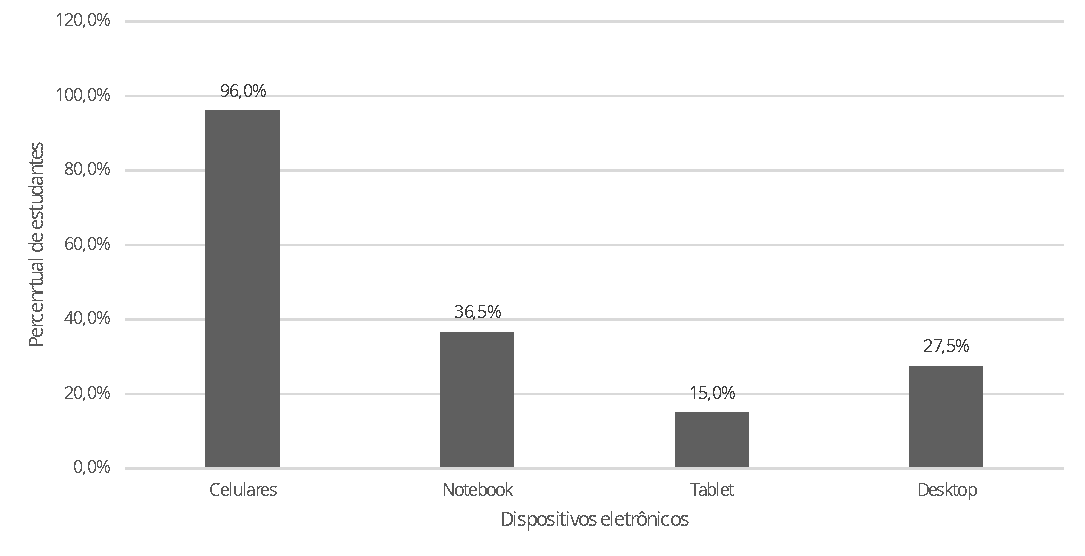
\includegraphics[width=\linewidth]{Graf1.pdf}
\caption{Acesso a dispositivos eletrônicos em casa.}
\label{fig1}
\source{Elaboração própria, a partir dos dados gerados.}
\end{minipage}
\end{figure}

Os dados revelam, portanto, que a internet é acessada por meio de celular pela ampla maioria dos adolescentes. Essa constatação confirma pesquisa realizada por entidades associadas que publicaram, em 2023, estudo relacionado ao uso de TIC por crianças e adolescentes brasileiros, a fim de compreender suas práticas, os riscos e as oportunidades decorrentes desse uso. Essa investigação explicita que, em 2023, 97\% desse público utilizava celular; 38\%, computador; e apenas 22\%, \textit{tablet} \cite{centro_regional_de_estudos_para_o_desenvolvimento_da_sociedade_da_informacao_tic_2023}.

O questionário também solicitou aos adolescentes que destacassem quanto tempo do seu dia permaneciam conectados à internet. Quase 44\% dos estudantes afirmaram permanecer mais de 5h diárias; 17,5\%, de 3h a 4h diárias; 11\%, de 2h a 3h. Esses dados estão intrinsecamente relacionados ao fato de que 96\% desses estudantes têm um celular com acesso à internet própria e quase 91\% levam o aparelho para escola.

É importante frisar que os adolescentes estão na escola das 7h às 16h40min, ou seja, provavelmente, parte significativa do tempo conectado ocorre no ambiente escolar. Na instituição onde a pesquisa foi desenvolvida, há uma rede wi-fi aberta aos estudantes, mas, geralmente, é possível conexão somente no pátio; não há rede wi-fi nas salas de aula. Entretanto, a ausência de wi-fi na maior parte dos espaços não impossibilita o acesso às redes durante as aulas, visto que quase metade dos estudantes, 46,5\%, utiliza rede 4G, ainda com a possibilidade de compartilhar dados móveis.

Nas conversas com esses adolescentes, alguns justificam suas horas na internet pela ``rolagem infinita'', com perda de percepção do tempo gasto. Vão-se horas no ato de navegar em plataformas e/ou em aplicativos de jogos \textit{on-line}. No prólogo do livro \textit{Irresistível: por que você é viciado em tecnologia e como lidar com ela}, o psicólogo \textcite{alter_irresistivel:_2018} cita Greg Houchmuth, um dos engenheiros fundadores do Instagram, que confessa que criou uma máquina de viciar:

\begin{quote}
    ``Sempre tem outra hashtag para clicar'', disse Hochmuth. ``Então a rede adquire vida própria, como um organismo, e as pessoas podem ficar obcecadas.'' O Instagram, como tantas outras plataformas de mídia social, é um poço sem fundo. O feed do Facebook é infinito; a Netflix passa automaticamente ao episódio seguinte; o Tinder encoraja os usuários a continuar passando o dedo de foto em foto em busca de uma opção melhor \cite[p.~10-11]{alter_irresistivel:_2018}.
\end{quote}

A própria arquitetura dessas plataformas digitais propicia o aumento do tempo de tela, posto que o sistema de ``rolagem infinita'' promete entregar sempre a última novidade, fazendo, dessa forma, com que sejamos trabalhadores explorados pela nova face do capital em sua era pós-fordista, sempre avaliando, curtindo, compartilhando, enquanto que os lucros das \textit{big-tecs} alcançam números astronômicos. De acordo com \textcite[p.~11]{alter_irresistivel:_2018},

\begin{quote}
    [os] usuários se beneficiam desses aplicativos e sites, mas também têm dificuldade em usá-los com moderação. Segundo Tristan Harris, especialista em ``ética de design'', o problema não é a falta de força de vontade das pessoas; a questão é que ``existem mil profissionais do outro lado da tela cujo trabalho é derrubar suas barreiras de autocontrole''.
\end{quote}

O tempo gasto poderia se constituir sozinho em um grande problema, mas, conforme \textcite{desmurget_fabrica_2023}, a questão é mais complexa, já que as práticas de crianças e adolescentes não se orientam no sentido de utilizações mais nitidamente positivas, ao contrário, há um caráter nocivo diante do arsenal disponível nas telas. O autor, após confrontar dados de várias pesquisas ao redor do mundo, concluiu que quanto mais aumenta o tempo de tela, mais o desempenho escolar diminui.

O uso do celular na escola, sem relação com as práticas pedagógicas, tem sido recorrente e tem provocado discussões em todas as etapas de ensino. No contexto dos estudantes desta pesquisa, a proibição do uso do celular consta no Regimento Escolar, com exceção nos casos de utilização para fins pedagógicos; bem como o uso é vedado aos professores em alguns espaços, entretanto, essa determinação não tem efeito prático.

\textcite{desmurget_fabrica_2023} cita estudos que mostram o quanto é difícil resistir ao ``chamado do celular'':

\begin{quote}
    Uma população diversa de alunos (do ensino fundamental à universidade) foi observada durante uma sessão de trabalho de quinze minutos. Em média, os participantes passaram somente 10 minutos estudando. Apesar da presença inquisidora de um pesquisador, eles não conseguiram ultrapassar 6 minutos de concentração antes de se lançarem esfomeados sobre seus aparelhos eletrônicos \cite[p.~185]{desmurget_fabrica_2023}.
\end{quote}

O autor, um neurocientista cognitivo, analisa outros casos semelhantes e conclui que nossa performance intelectual está sendo bastante afetada pela presença excessiva das telas, sobretudo nas escolas. Nossa atenção, nossa concentração e o nosso desempenho intelectual ficam bastante prejudicados.

Outro aspecto discutido por Desmurget é a importância de desmistificar a ideia de que o jovem da atualidade consegue realizar inúmeras tarefas ao mesmo tempo. Segundo ele, essa ``farsa pseudocientífica'' \cite[p.~123]{desmurget_fabrica_2023} convence os próprios estudantes de que conseguem acompanhar uma aula ou fazer seus deveres de casa enquanto assistem a videoclipes ou séries, ``surfam'' nas redes sociais e/ou trocam mensagens de texto. Uma falácia, já que nosso cérebro não direciona sua atenção para todas essas tarefas concomitantemente, apenas uma por vez. Conforme o autor, não há pesquisas científicas que sustentem essa tese de ``nativos digitais'', ao contrário, há objeção por parte da comunidade científica ao conceito, já que

\begin{quote}
    [...] a nova geração supostamente designada por esses termos não existe. É inegável que podemos sempre encontrar, procurando com afinco, alguns indivíduos cujos hábitos de consumo correspondem vagamente ao estereótipo esperado do geek supercompetente com os olhos grudados nas suas telas; mas esses modelos tranquilizadores são mais uma exceção do que uma regra. Em seu conjunto, a suposta ``geração Internet'' se assemelha bem mais a ``uma reunião de minorias'' do que a um grupo homogêneo \cite[p.~21]{desmurget_fabrica_2023}.
\end{quote}

Apesar de essa geração utilizar de forma recreativa as tecnologias digitais com muito êxito, apresenta dificuldades no domínio de competências de informática mais rudimentares, desde ligar um computador \textit{desktop} a formatar um texto em editor digital – práticas essas observadas em nosso dia a dia como professores. Assim, podemos afirmar que o exacerbado tempo conectado não se traduz em domínio das potencialidades dos recursos tecnológicos, bem como das possibilidades de produção de conhecimentos.

\section{Redes sociais}\label{sec-formato}
As redes sociais fazem parte do nosso dia a dia. Em nosso estudo, ao investigar as práticas mais recorrentes na internet, constatamos que 84,5\% dos estudantes acessam as redes sociais; 74,5\% utilizam para pesquisas escolares; 67,5\% acessam plataformas de músicas; 51\% jogam \textit{on-line}; 47,5\% assistem a vídeos no YouTube; e 42\% consomem conteúdos de plataformas de \textit{streaming}, conforme a \Cref{fig2}.

\begin{figure}
\centering
\begin{minipage}{0.85\linewidth}
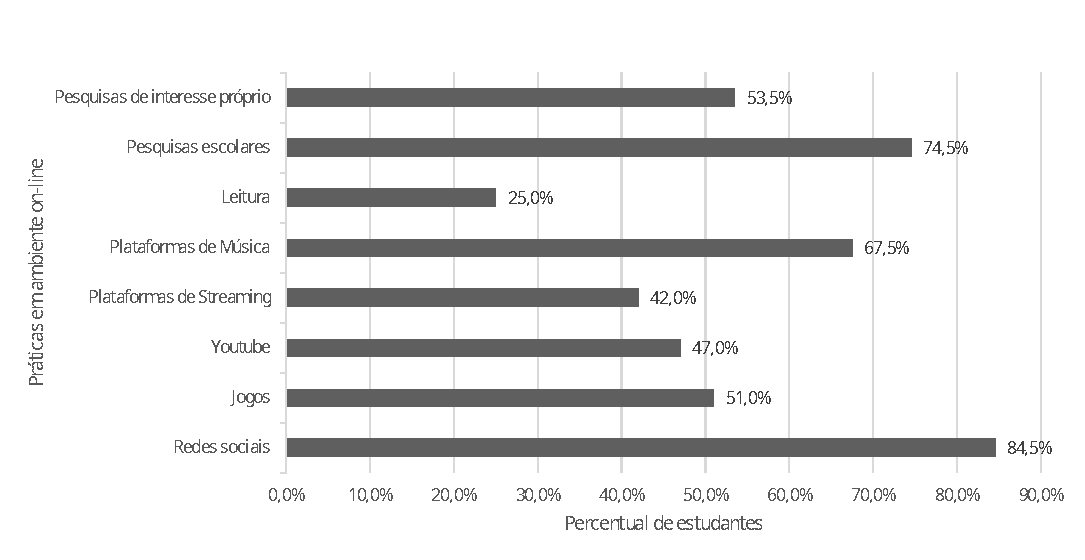
\includegraphics[width=\linewidth]{Graf2.pdf}
\caption{Práticas mais recorrentes dos estudantes na internet.}
\label{fig2}
\source{Elaboração própria, a partir dos dados gerados.}
\end{minipage}
\end{figure}

Esses dados confirmam que os estudantes estão imersos nas dinâmicas de funcionamento das redes sociais. Aos perguntarmos quais redes sociais acessavam, o Instagram foi a mais citada: 94\%. Na sequência, aparecem WhatsApp (90\%), TikTok (72\%) e YouTube (61,5\%). O Facebook e o X (antigo Twitter) foram citados, respectivamente, por 24\% e 23,5\% dos estudantes. Menos acessados, o Telegram (14\%), o Kwai (11\%) e o Snapchat (5\%) também foram mencionados. Esses dados confirmam a pesquisa \textit{TIC Kids Online Brasil} 2023, a qual apresenta que, do total de usuários da internet de 9 a 17 anos, 36\% utilizam o Instagram; 29\%, o YouTube; 27\%, o TikTok; e 2\%, o Facebook \cite[p.~11]{centro_regional_de_estudos_para_o_desenvolvimento_da_sociedade_da_informacao_tic_2023}.

Por um lado, essas redes sociais nos oferecem a hiperconectividade com o mundo, de maneira a se ``venderem'' como ambientes ``abertos'' para todos; por outro, dão novos contornos ao capitalismo em sua forma neoliberal, de maneira a transformar o sujeito numa empresa que precisa ser produtiva e gerar lucros, por meio da produção de conteúdos e do retorno através de \textit{likes} e compartilhamentos. Conforme \textcite{lanier_dez_2018}, a principal função das redes sociais é promover engajamento, manter os sujeitos cada vez mais conectados e expostos à publicidade, consequentemente, gerar lucro. Na esteira desse pensamento, \textcite{vietri_community_2019} destaca que quando um serviço é gratuito, o produto é o consumidor.

Além disso, atuam na produção da subjetividade contemporânea, pautada, conforme o filósofo \textcite{han_sociedade_2015}, na sociedade do desempenho, na qual e para qual os corpos devem sempre apresentar a melhor versão de si, do sucesso, da produção, tudo devidamente registrado e compartilhado por nossos \textit{smartphones}. Nessa lógica, nas  palavras do filósofo \textcite[p.~21]{bauman_vigilancia_2013},

\begin{quote}
    [os] adolescentes equipados com confessionários eletrônicos portáteis não passam de aprendizes treinando a (e treinando na) arte de viver numa sociedade confessional; uma sociedade que se destaca por eliminar a fronteira que antes separava o privado do público, por fazer da exposição pública do privado uma virtude e uma obrigação pública, e por varrer da comunicação pública qualquer coisa que resista a ser reduzida a confidências privadas juntamente com aqueles que se recusam a confidenciá-las.
\end{quote}

Pelo que nos diz o autor, rompem-se os limites entre o público e o privado, exaspera-se o individualismo e a autoexposição. Nessa perspectiva, \textcite{faustino_colonialismo_2023} afirmam que

\begin{quote}
    [...] não se tira foto do treino, mas, sim, treina-se para tirar foto. Em um cenário que já podemos nomear de biopunk, adolescentes querem produzir na carne o que os filtros do Instagram criam no ciberespaço, em realidade aumentada. Assim, o uso abusivo de plásticas e substâncias estéticas torna-se imperativo para sustentar a autoimagem \cite[p.~159-160]{faustino_colonialismo_2023}.
\end{quote}

A escola não está fora desse cenário ``biopunk'' \cite{faustino_colonialismo_2023}, de maneira que tais discursos e práticas também circulam na instituição. Como constatamos, os adolescentes do Ensino Médio estão expostos às ideologias disseminadas nas redes sociais, bem como contribuem, mesmo que inconscientemente, com a manutenção e a disseminação dessa lógica de produção.

\section{Práticas de pesquisa em ambiente digital}\label{sec-modelo}
Além de acessarem redes sociais, quase 75\% dos estudantes usam a internet para pesquisas escolares em sites de busca. Esses mecanismos são sistemas de recuperação de informações com a finalidade de contribuir para o acesso a dados armazenados em ambientes digitais. Funcionam por meio de rastreamento da Web e de indexação de páginas que serão retornadas ao usuário, através de uma interface com resultados e \textit{links} de acesso \cite{caldeira_o_2015}.

Apesar da diversidade de buscadores existentes, o Google é o mais adotado pelos brasileiros – fato que tornou a expressão popularmente difundida ``dar um Google'' sinônimo de ``pesquisar''. Entre os participantes desta investigação, 75\% citaram esse buscador quando questionados sobre qual site utilizam para pesquisas escolares, e pouco mais de 60\% recorrem a ele para pesquisas de interesse próprio. Essas estatísticas são resultados de duas perguntas distintas sobre pesquisa na internet, uma direcionada à escolar e outra à de interesse próprio. Constatamos que os estudantes, geralmente, associam pesquisas solicitadas pelo professor à busca no Google, como um recurso consolidado. Já para pesquisas de interesse próprio, recorrem, também, às redes sociais, conforme quase 23\% informaram.

Outro resultado significativo foi o baixo percentual de estudantes que dizem utilizar ferramentas de Inteligência Artificial, como ChatGPT e/ou aplicativo LuzIA, em pesquisas escolares: apenas 3\%. Esse dado reforça a fragilidade da concepção muito difundida de estudantes da atual geração como ``nativos digitais'', visto que uma minoria conhece e usa IA nas práticas escolares, por exemplo.

Questionamos os estudantes, também, sobre a preferência pelo formato do conteúdo ao fazerem uma pesquisa na internet. Quase 80\% pesquisam ``textos''; 12\% buscam ``vídeos'' e 9\% selecionam ``imagens''. Entretanto, nas práticas de sala de aula, percebemos um fenômeno recorrente: eles pesquisam por textos, resumos, na aba ``imagem'' do Google. Por exemplo, em turmas distintas, solicitamos que os estudantes pesquisassem o tópico ``funções da linguagem''. Todos, primeiramente, abriram a página Google, pesquisaram pela expressão ``funções da linguagem'' e, em seguida, quase a totalidade usou o recurso ``imagem'', em destaque na \Cref{fig3}:

\begin{figure}
\centering
\begin{minipage}{\linewidth}
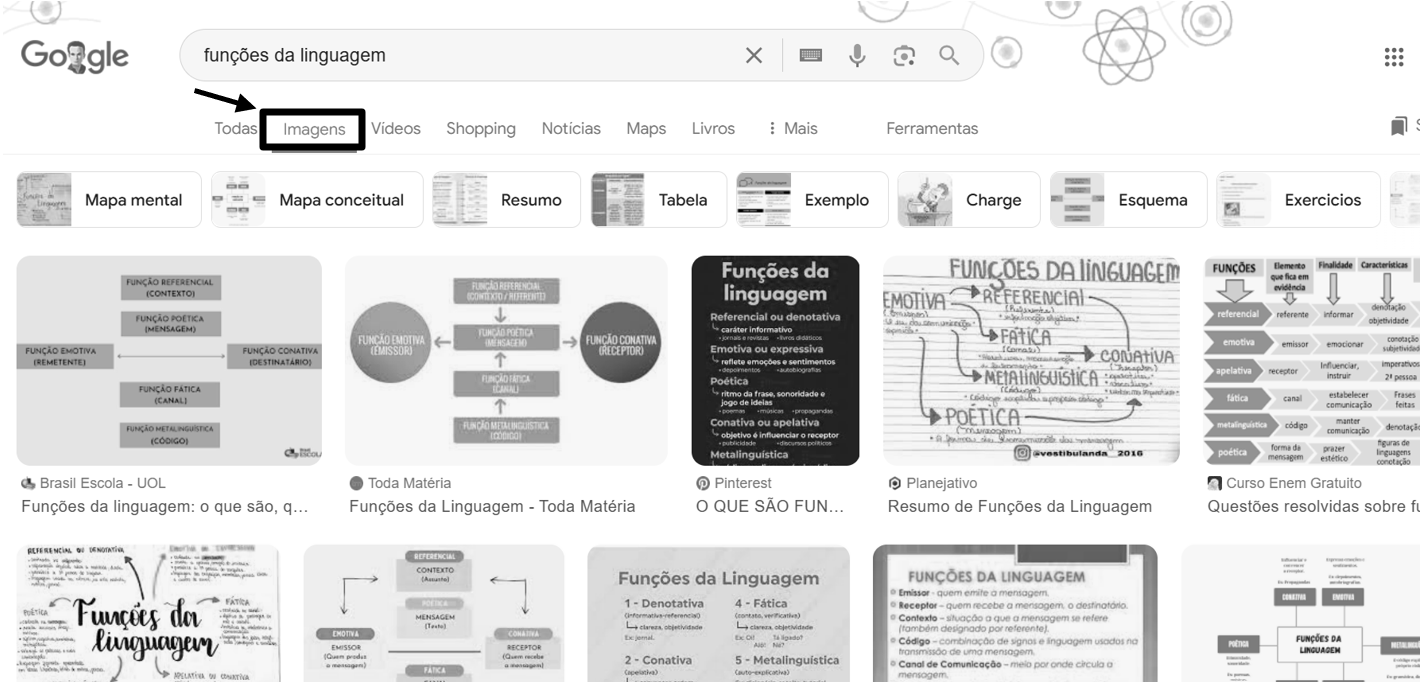
\includegraphics[width=\linewidth]{Fig1.png}
\caption{Exemplo de tela da pesquisa dos estudantes.}
\label{fig3}
\source{Produção própria. \textit{Print} da página de pesquisa Google.}
\end{minipage}
\end{figure}

Os estudantes reproduziram em seus cadernos a sistematização do conteúdo em figuras, quadros e mapas conceituais produzidos e disponibilizados por outras pessoas, geralmente, optando por imagens com menos conteúdo verbal.
Ainda sobre as práticas de pesquisa, investigamos como os estudantes mobilizam as informações e os \textit{links} retornados após a pesquisa no buscador. Quase 52\% deles afirmaram que copiam apenas as informações sugeridas pelo ``resumo do Google'', recurso em destaque na \Cref{fig4}. 

\begin{figure}
\centering
\begin{minipage}{\linewidth}
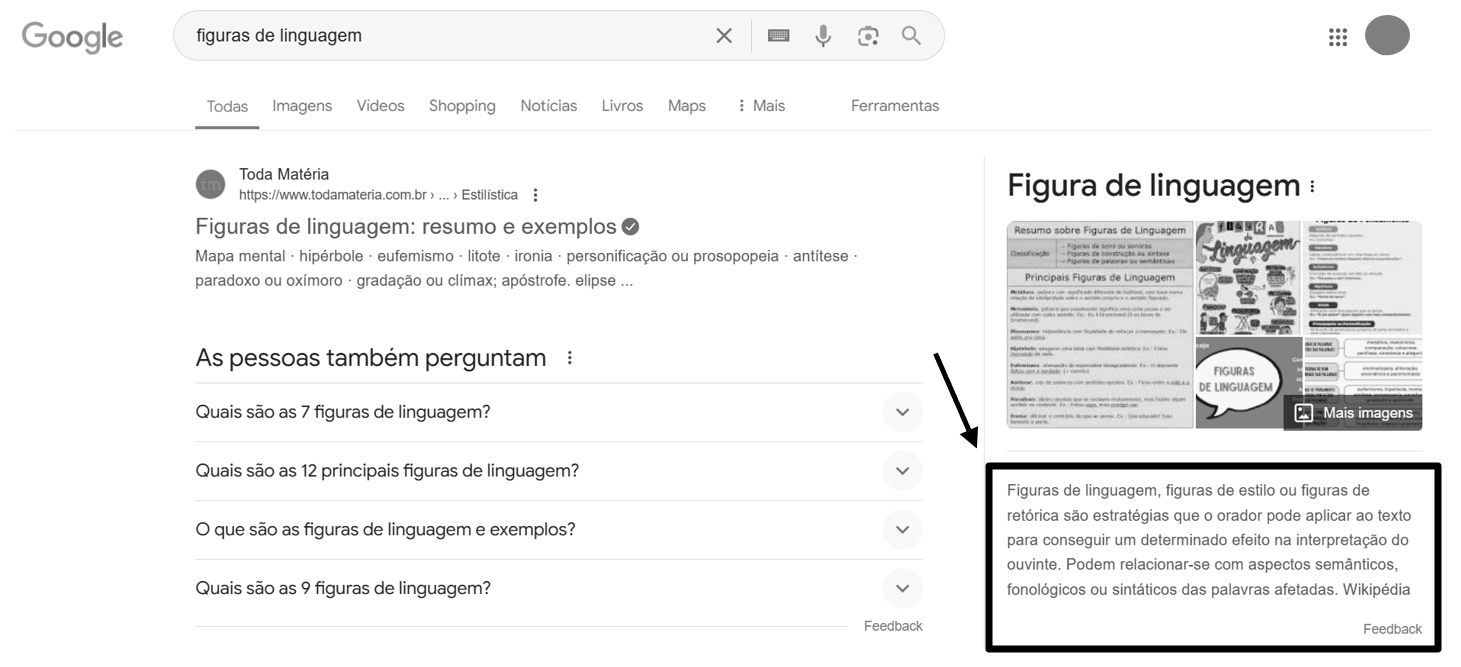
\includegraphics[width=\linewidth]{Fig2.png}
\caption{Exemplo de tela da pesquisa dos estudantes.}
\label{fig4}
\source{Produção própria. \textit{Print} da página de pesquisa Google.}
\end{minipage}
\end{figure}

Já 37\% afirmaram que copiam informações de diversos sites sugeridos pelo buscador; 8\% contentam-se em clicar no primeiro \textit{link} que aparece e 5\% trabalham com informações de sites patrocinados. Esses dados podem nos ajudar a refletir sobre a necessidade de se ensinar práticas de pesquisa na internet. Nesse sentido, cabe pensarmos, também, em como as informações são organizadas pela principal ferramenta de busca utilizada pelos estudantes; no site da Google, na página ``Como resultados são gerados automaticamente'', a empresa informa:

\begin{quote}
    Com a grande quantidade de informações disponíveis, encontrar o que você precisa seria quase impossível sem uma ajudinha. Os sistemas de classificação do Google são projetados para fazer exatamente isso: organizar centenas de bilhões de páginas da Web e outros tipos de conteúdo no índice da Busca e oferecer os resultados mais relevantes e úteis em uma fração de segundo \cite{google_como_nodate}.
\end{quote}

Nessa página, não há outras informações sobre os critérios de seleção dos \textit{links} que são apresentados. A ferramenta é descrita quase como uma entidade metafísica, que ``generosamente'' seleciona as informações solicitadas pelos usuários. No entanto, não ``existe \textit{software} sem \textit{hardware}'', pois ``[…] por mais que sejam intangíveis, os softwares são produzidos pelo trabalho humano – não dão em árvores […]'' \cite[p.~112]{faustino_colonialismo_2023}. Isso implica entender que as tecnologias digitais são fruto e pomar do contexto sócio-histórico no qual são desenvolvidas. Em outras palavras, essas ferramentas estão a serviço dos interesses políticos e ideológicos das grandes corporações.

\section{Por uma educação crítica}\label{sec-organizacao}
A escola é uma instituição fundamental na sociedade. É um importante espaço de aprendizagem, de convivência e é nela que circulam discursos vários, antagônicos, muitas vezes. Nessas duas direções, uma educação crítica se faz necessária.

Como espaço de convivência, a escola ensina a relacionar-se com o outro, ensina a compreender o outro como diferente, não só fisicamente, mas na forma de pensar e de agir. Conhecer e respeitar outras cores de pele, outras sexualidades e gêneros, outras formas de ser, é uma aprendizagem que se faz na convivência de sala de aula e com outras turmas, com pares, com autoridades, com parecidos e diferentes em relações simétricas e assimétricas. Aprender a estabelecer limites para si mesmo e para o outro, visando a uma convivência saudável, exige relacionamentos presenciais, porque não podem ser ensinados apenas discursivamente. A escola, então, precisa investir em projetos coletivos de convivência, em que o relacionamento entre toda a comunidade escolar seja mais afetivo, humano e pautado pelo querer bem aos estudantes, afinal, é ``preciso descartar como falsa a separação radical entre seriedade docente e afetividade […] porque a afetividade não se acha excluída da cognoscibilidade'' \cite[p.~138]{freire_pedagogia_2011}. É justamente na contramão dessa filosofia do ``educar como um ato de amor'' que alguns defendem propostas limitadoras, de isolamento ou de filosofia única que não contribuem para a formação humana na e para a diversidade, ao contrário, exacerbam o individualismo e a competição. A diversidade está na escola em todas as suas formas de existência e aprender a lidar com ela é um trabalho essencial na formação das (futuras) gerações.

Além de promover relações humanas amorosas, a escola precisa investir ainda mais na criticidade, em leituras críticas da realidade. Se é fato que a internet participa da nossa vida, e o celular é um ``objeto'' onipresente no nosso dia a dia, o questionamento do seu uso, do tempo de tela e das práticas ali efetivadas por todos nós, ainda mais por adolescentes do Ensino Médio, faz-se necessário e urgente.

A leitura crítica da realidade engloba um leque de questões inter-relacionadas. O começo está na desnaturalização da atual realidade (social, cultural e histórica), ou seja, a compreensão de que as gigantes da tecnologia visam ao lucro, e nós, involuntariamente, nos transformamos em consumidores e trabalhadores de ``conteúdos'', através dos nossos ``cliques'' e compartilhamentos. 

Nessa perspectiva, discutir com os estudantes a existência de outras possibilidades de uso de sistemas/\textit{softwares} livres de informática torna-se uma maneira de resistência às gigantes da tecnologia. Ter conhecimento da luta travada pelo grupo liderado por Stallman, um dos pioneiros nessa área, para desenvolver programas em que o usuário, ``em vez de se submeter a um \textit{software}, [tem] sempre a possibilidade de modificá-lo, sem ser forçado a pedir autorização para adaptá-lo a suas necessidades'' \cite[p.~131]{loveluck_redes_2018}, torna-se essencial para ampliar horizontes de conhecimento e ajudar o adolescente a perceber que não há obrigatoriedade de vinculação a empresas que desenvolvem \textit{softwares} em formato ``proprietário''. \textcite[p.~6]{gonsales_educacao_2020} sistematizam as vantagens desses \textit{softwares} de código aberto, conforme a \Cref{fig5}:

\begin{figure}
\centering
\begin{minipage}{0.75\linewidth}
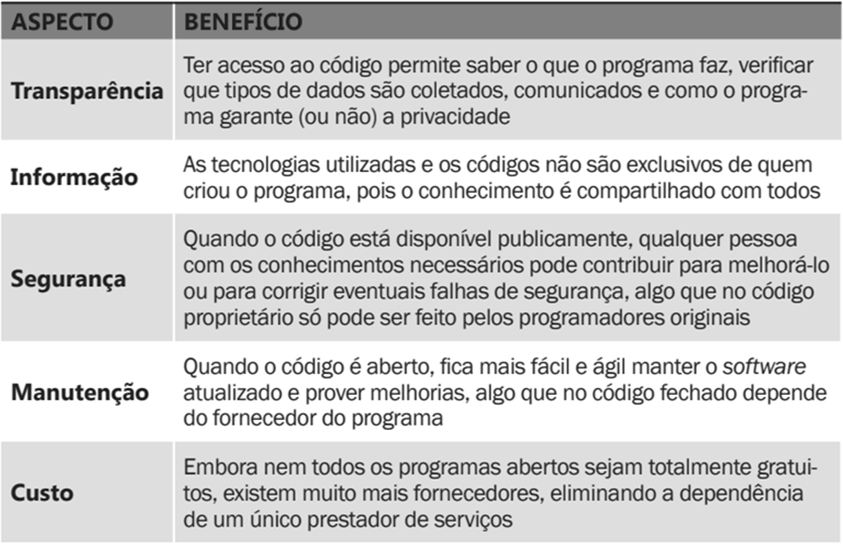
\includegraphics[width=\linewidth]{Fig3.png}
\caption{Sistematização dos aspectos e benefícios do uso de \textit{softwares} de código aberto.}
\label{fig5}
\source{\textcite[p.~6]{gonsales_educacao_2020}.}
\end{minipage}
\end{figure}

Assim, a proposta de utilização de \textit{softwares} livres articula um conjunto de ideias que buscam preservar os direitos digitais também de acesso à informação e o direito à privacidade. Essa é uma importante discussão para ser feita nas escolas, visto que uma parcela significativa da sociedade desconhece a existência dessas possibilidades.

Discutir com nossos adolescentes o que consumimos e produzimos nas redes sociais também é fundamental. Nossos tempos são marcados, como pontuamos anteriormente, pela autoexposição, pela publicização de questões privadas, pela busca do corpo ``perfeito'', pelo mundo ``feliz'' que emerge das postagens, e paradoxalmente pelo adoecimento psicológico de uma geração. Textos que ajudem o estudante a refletir para além da aparência dos fatos, que apresentem a ``contrapalavra'', um outro discurso, são essenciais para a formação do sujeito. O discurso único, hegemônico, tende a aprisioná-lo em uma ``bolha''. Já a apresentação de perspectivas contra-hegemônicas tendem a criar ``conflito'', ``embate''. O resultado do enfrentamento é a tomada de posição e a produção da própria palavra \cite{bakhtin_estetica_2003}. Sujeitos críticos são aqueles que confrontam dizeres, que leem as linhas e as entrelinhas, que não descontextualizam informações ou que buscam recontextualizá-las, porque sabem que elementos de ancoragem do discurso são essenciais para compreendê-lo. Sujeitos críticos buscam informações em múltiplas fontes \cite{coscarelli_leitura_2017}, não se contentam em clicar no primeiro site que aparece em navegadores; também não se contentam com resumos produzidos por IA. Sujeitos críticos guiam-se pela ``curiosidade epistemológica'' \cite{freire_pedagogia_2011}.

Na esteira desse pensamento, proibir o uso de celular na escola não é solução, como defendem alguns pais e professores. A sua utilização ``livre'', sem regras, igualmente nada resolverá. Precisamos de encontros de discussão e acordos claros: com quais objetivos poderemos utilizar o celular na escola e por quanto tempo? Pontos de concordância entre professores, estudantes, pais, direção e funcionários serão a ``lei'' de sua utilização na escola. Além disso, todos precisarão se adequar ao combinado, do contrário, ensinaremos, indiretamente, que combinados não precisam ser seguidos, aspecto tão pernicioso quanto a proibição.

Enfim, uma educação crítica, que abarque a convivência com a diversidade e proporcione a leitura crítica da palavramundo \cite{freire_importancia_1989}, pode se constituir no contraponto do que é vivido, no contraponto da cultura do individualismo e da competição, e a escola é uma instituição importantíssima nesse sentido.

\section{Considerações finais}\label{sec-organizacao-latex}
Os dados analisados na nossa pesquisa comprovam que o adolescente tem acesso ao celular e o utiliza muitas horas por dia, inclusive no espaço escolar. Acessa o Instagram e o WhatsApp majoritariamente e pouco utiliza o aparelho para pesquisas escolares. Quando o faz, consulta textos na aba ``imagem'' do Google, sua principal estratégia de busca por conhecimento na internet. 
As grandes corporações massificam o uso de redes sociais, viciam o adolescente – não só ele -, porque obtêm lucro. Para elas, não há problema se os adolescentes estão colhendo frutos amargos nos seus estudos, ou se estão cada vez mais adoecidos psicologicamente. A lógica do capital é dominante, assume contornos distintos para continuar explorando corpos e mentes a favor de seus objetivos. Em uma sociedade injusta, não há ética nas relações comerciais.

A escola precisa ser a instância, por excelência, de reflexão do que o adolescente está vivendo, de como está se sentindo, diante da quantidade absurda de conteúdos disponíveis, na aparente democracia do ``tudo postar''. Como já dizia Freire, em 1984, ``a máquina está a serviço de quem?'' deve ser a pergunta-chave da educação crítica. Isso não significa ``demonizar'' ou desconsiderar os benefícios das tecnologias na vida contemporânea; nem minimizar as potencialidades dos usos nas práticas pedagógicas, mas ampliar as discussões no sentido de não naturalizar os impactos negativos ou os modos de operar a serviço do capital.

Nesse sentido, a internet precisa ser regulamentada. As grandes corporações precisam ser responsabilizadas pelo que circula nas suas plataformas e aplicativos. O argumento da ``liberdade de expressão'' tem sido utilizado pela ultradireita do nosso país para justificar a não regulamentação. No entanto, a liberdade de expressão deve ser limitada na justa medida em que a ``preservação da vida'' seja a baliza. Viver em sociedade exige acordos, e o limite do que pode ser dito ou feito está na ``preservação da vida'' (do outro). A regulamentação das mídias digitais fará com que aplicativos e/ou redes sociais redefinam a apresentação de conteúdos, já que não podem continuar sendo determinados pelas ``curtidas'' dos usuários. Da mesma forma, as grandes empresas de tecnologia não devem ter livre acesso aos nossos dados, às nossas formas de vida, traduzidos em algoritmos que geram ainda mais demandas de consumo de produtos e de conteúdos.

A sociedade do desempenho \cite{han_sociedade_2015} está exigindo mudanças na direção oposta a ela e ao que representa na formação dos adolescentes. Estabelecer relações mais humanas e afetivas nos contatos presenciais, como dissemos, trabalhar pelo reconhecimento do outro como um sujeito com os mesmos direitos de cada um de nós, também é fundamental. Vale lembrar que nosso país criou o Estatuto da Criança e do Adolescente, em 1990, uma tentativa de imputar aos adultos as necessárias ações visando à proteção desses sujeitos \cite{brasil_estatuto_1990}. Mais de trinta anos após a sua promulgação, ainda estamos muito longe de proteger os adolescentes, ao contrário, exacerbamos a ``não proteção'' da vida nas/das telas.


\section{Finciamento}
O presente trabalho foi realizado com apoio da Coordenação de Aperfeiçoamento de Pessoal de Nível Superior – Brasil (CAPES) - Código de Financiamento 001 "This study was financed in part by the Coordenação de Aperfeiçoamento de Pessoal de Nível Superior – Brasil (CAPES) - Finance Code 001.

\printbibliography\label{sec-bib}
%conceptualization,datacuration,formalanalysis,funding,investigation,methodology,projadm,resources,software,supervision,validation,visualization,writing,review
\begin{contributors}[sec-contributors]
\authorcontribution{Marcelo Rodrigues de Lima}[conceptualization,datacuration,formalanalysis,investigation,methodology,projadm,validation,visualization,writing,review]
\authorcontribution{Pedro Henrique Souza da Silva}[conceptualization,formalanalysis,investigation,methodology,projadm,validation,visualization,writing,review]
\authorcontribution{Adriane Teresinha Sartori}[conceptualization,formalanalysis,investigation,methodology,projadm,validation,visualization,writing,review]
\end{contributors}
\end{document}
